\documentclass[]{article}
\usepackage{lmodern}
\usepackage{amssymb,amsmath}
\usepackage{ifxetex,ifluatex}
\usepackage{fixltx2e} % provides \textsubscript
\ifnum 0\ifxetex 1\fi\ifluatex 1\fi=0 % if pdftex
  \usepackage[T1]{fontenc}
  \usepackage[utf8]{inputenc}
\else % if luatex or xelatex
  \ifxetex
    \usepackage{mathspec}
  \else
    \usepackage{fontspec}
  \fi
  \defaultfontfeatures{Ligatures=TeX,Scale=MatchLowercase}
\fi
% use upquote if available, for straight quotes in verbatim environments
\IfFileExists{upquote.sty}{\usepackage{upquote}}{}
% use microtype if available
\IfFileExists{microtype.sty}{%
\usepackage{microtype}
\UseMicrotypeSet[protrusion]{basicmath} % disable protrusion for tt fonts
}{}
\usepackage[margin=1in]{geometry}
\usepackage{hyperref}
\hypersetup{unicode=true,
            pdftitle={LDA妯″瀷鎻忚堪\textgreater{}},
            pdfauthor={鐜嬫煶鐩\textless{}88\textgreater{}},
            pdfborder={0 0 0},
            breaklinks=true}
\urlstyle{same}  % don't use monospace font for urls
\usepackage{graphicx,grffile}
\makeatletter
\def\maxwidth{\ifdim\Gin@nat@width>\linewidth\linewidth\else\Gin@nat@width\fi}
\def\maxheight{\ifdim\Gin@nat@height>\textheight\textheight\else\Gin@nat@height\fi}
\makeatother
% Scale images if necessary, so that they will not overflow the page
% margins by default, and it is still possible to overwrite the defaults
% using explicit options in \includegraphics[width, height, ...]{}
\setkeys{Gin}{width=\maxwidth,height=\maxheight,keepaspectratio}
\IfFileExists{parskip.sty}{%
\usepackage{parskip}
}{% else
\setlength{\parindent}{0pt}
\setlength{\parskip}{6pt plus 2pt minus 1pt}
}
\setlength{\emergencystretch}{3em}  % prevent overfull lines
\providecommand{\tightlist}{%
  \setlength{\itemsep}{0pt}\setlength{\parskip}{0pt}}
\setcounter{secnumdepth}{0}
% Redefines (sub)paragraphs to behave more like sections
\ifx\paragraph\undefined\else
\let\oldparagraph\paragraph
\renewcommand{\paragraph}[1]{\oldparagraph{#1}\mbox{}}
\fi
\ifx\subparagraph\undefined\else
\let\oldsubparagraph\subparagraph
\renewcommand{\subparagraph}[1]{\oldsubparagraph{#1}\mbox{}}
\fi

%%% Use protect on footnotes to avoid problems with footnotes in titles
\let\rmarkdownfootnote\footnote%
\def\footnote{\protect\rmarkdownfootnote}

%%% Change title format to be more compact
\usepackage{titling}

% Create subtitle command for use in maketitle
\newcommand{\subtitle}[1]{
  \posttitle{
    \begin{center}\large#1\end{center}
    }
}

\setlength{\droptitle}{-2em}
  \title{LDA妯″瀷鎻忚堪\textgreater{}}
  \pretitle{\vspace{\droptitle}\centering\huge}
  \posttitle{\par}
  \author{鐜嬫煶鐩\textless{}88\textgreater{}}
  \preauthor{\centering\large\emph}
  \postauthor{\par}
  \date{}
  \predate{}\postdate{}

\usepackage{ctex}

\begin{document}
\maketitle

\section{数据获取}

网站\href{http://chuansong.me/}{传送门}
转载了各大微信公众号的历史文章。我们从该网站上随机抽取三个关注人数较多的娱乐八卦公众号,抓取2016年4月中旬至2017年2月中旬的所有历史文章,及其阅读数与点赞数等信息,共计1953条记录作为我们的语料库。

\section{理论}

\subsection{LDA模型}\label{lda}

潜在狄利克雷分布(Latent Dirichlet
allocation,LDA)主题模型,是文本挖掘中著名的生成概率模型。它由David M.
Blei、Andrew Y. Ng、Michael I. Jordan在2013年提出。

\subsubsection{记号:}

\begin{enumerate}
\def\labelenumi{\arabic{enumi}.}
\item
  一个词语是该离散数据中最基本的单位,词典中所有词语由 \({1,2,...,V}\)
  索引。每个词语可由一个单位基向量表示,即词典中的第 \(v\) 个词表示为
  \(V\) 维向量 \(w\) ,其中 \(w^v=1\quad w^u=0,u\neq v\) ;
\item
  一篇具有 \(N\) 个词的文档记为词序列 \(\vec w_n=(w_1,w_2,...,w_N)\)
  ,其中 \(w_n\) 是序列中的第n个词语;
\item
  \(M\) 篇文档组成的语料库记为
  \(D=\{{\vec w}_1,{\vec w}_2,...,{\vec w}_M\}\) 。
\end{enumerate}

\subsection{DGP:}\label{dgp}

LDA是一个层次贝叶斯模型,它的基本思想是:一篇文章可能具有多个主题,而文档的主题分布服从一个潜在的狄利克雷分布,而每一个主题代表一种词语分布,即一篇文档的生成服从以下步骤:

\begin{enumerate}
\def\labelenumi{\arabic{enumi}.}
\tightlist
\item
  选择 \(N \sim Poission(\xi)\) ;
\item
  选择 \(\theta\sim Dir(\alpha)\) ;
\item
  对于N个词中的每一个词语 \(w_n\) :
\end{enumerate}

\begin{itemize}
\tightlist
\item
  选择其来自于哪一个主题 \(z_n\sim Multinomial(\theta)\) ;
\item
  从多项式条件分布 \(p(w_n|z_n,\beta)\) 中生成一个词语w\_n。
\end{itemize}

其中假设主题数k(狄利克雷分布的维度)是已知且固定的;给定主题,词语的条件分布kxV维矩阵
\(\beta \qquad where \quad\beta_{ij}=p(w^j=1|z^i=1)\)
是未知非随机矩阵。文档长度N服从泊松分布,且与过程1.、2.独立。

结构可表述如下图????

\begin{figure}[htbp]
\centering
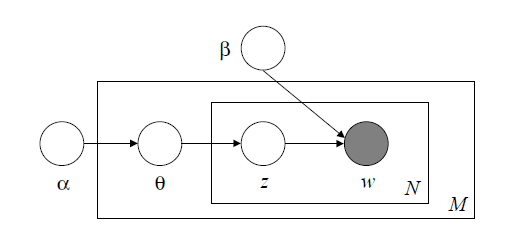
\includegraphics{lda1.PNG}
\caption{LDA结构图}
\end{figure}

需注意与简单狄利克雷-多项式分布聚类模型不同,LDA模型允许一个文档具有多个主题。

具有图{[}LDA结构图{]}所示结构的模型在贝叶斯方法中被称为层次模型(Gelman
et al., 1995),或条件独立层次模型(conditionally independent
hierarchical model, Kass and Steffey, 1989)。LDA参数
\(\alpha,\beta\)可以由经验贝叶斯方法进行估计。

\subsection{推断与参数估计}

LDA模型最终的目的是,给定文档,推断其潜在主题的后验分布:
\[p(\theta,\vec z|\vec w,\alpha,\beta)=\frac{p(\theta,\vec z,\vec w|\alpha,\beta)}{p(\vec w|\alpha,\beta)}\]
具体过程可以采用拉普拉斯逼近、变分近似法、MCMC方法计算。本文中我们采用MCMC方法,利用gibbs抽样近似计算后验分布。


\end{document}
